% Created by tikzDevice version 0.12.6 on 2024-06-25 17:18:43
% !TEX encoding = UTF-8 Unicode
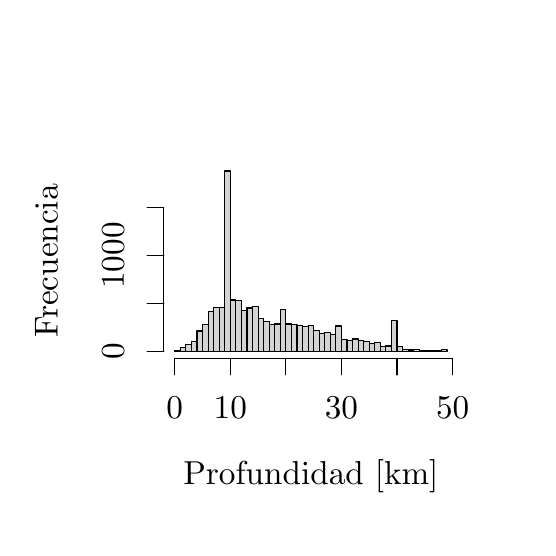
\begin{tikzpicture}[x=1pt,y=1pt]
\definecolor{fillColor}{RGB}{255,255,255}
\path[use as bounding box,fill=fillColor,fill opacity=0.00] (0,0) rectangle (180.67,180.67);
\begin{scope}
\path[clip] (  0.00,  0.00) rectangle (180.67,180.67);
\definecolor{drawColor}{RGB}{0,0,0}

\node[text=drawColor,anchor=base,inner sep=0pt, outer sep=0pt, scale=  1.20] at (102.34, 15.60) {Profundidad [km]};

\node[text=drawColor,rotate= 90.00,anchor=base,inner sep=0pt, outer sep=0pt, scale=  1.20] at ( 10.80, 96.34) {Frecuencia};
\end{scope}
\begin{scope}
\path[clip] (  0.00,  0.00) rectangle (180.67,180.67);
\definecolor{drawColor}{RGB}{0,0,0}

\path[draw=drawColor,line width= 0.4pt,line join=round,line cap=round] ( 53.14, 61.20) -- (153.55, 61.20);

\path[draw=drawColor,line width= 0.4pt,line join=round,line cap=round] ( 53.14, 61.20) -- ( 53.14, 55.20);

\path[draw=drawColor,line width= 0.4pt,line join=round,line cap=round] ( 73.22, 61.20) -- ( 73.22, 55.20);

\path[draw=drawColor,line width= 0.4pt,line join=round,line cap=round] ( 93.30, 61.20) -- ( 93.30, 55.20);

\path[draw=drawColor,line width= 0.4pt,line join=round,line cap=round] (113.38, 61.20) -- (113.38, 55.20);

\path[draw=drawColor,line width= 0.4pt,line join=round,line cap=round] (133.46, 61.20) -- (133.46, 55.20);

\path[draw=drawColor,line width= 0.4pt,line join=round,line cap=round] (153.55, 61.20) -- (153.55, 55.20);

\node[text=drawColor,anchor=base,inner sep=0pt, outer sep=0pt, scale=  1.20] at ( 53.14, 39.60) {0};

\node[text=drawColor,anchor=base,inner sep=0pt, outer sep=0pt, scale=  1.20] at ( 73.22, 39.60) {10};

\node[text=drawColor,anchor=base,inner sep=0pt, outer sep=0pt, scale=  1.20] at (113.38, 39.60) {30};

\node[text=drawColor,anchor=base,inner sep=0pt, outer sep=0pt, scale=  1.20] at (153.55, 39.60) {50};

\path[draw=drawColor,line width= 0.4pt,line join=round,line cap=round] ( 49.20, 63.80) -- ( 49.20,115.61);

\path[draw=drawColor,line width= 0.4pt,line join=round,line cap=round] ( 49.20, 63.80) -- ( 43.20, 63.80);

\path[draw=drawColor,line width= 0.4pt,line join=round,line cap=round] ( 49.20, 81.07) -- ( 43.20, 81.07);

\path[draw=drawColor,line width= 0.4pt,line join=round,line cap=round] ( 49.20, 98.34) -- ( 43.20, 98.34);

\path[draw=drawColor,line width= 0.4pt,line join=round,line cap=round] ( 49.20,115.61) -- ( 43.20,115.61);

\node[text=drawColor,rotate= 90.00,anchor=base,inner sep=0pt, outer sep=0pt, scale=  1.20] at ( 34.80, 63.80) {0};

\node[text=drawColor,rotate= 90.00,anchor=base,inner sep=0pt, outer sep=0pt, scale=  1.20] at ( 34.80, 98.34) {1000};
\end{scope}
\begin{scope}
\path[clip] ( 49.20, 61.20) rectangle (155.47,131.47);
\definecolor{drawColor}{RGB}{0,0,0}
\definecolor{fillColor}{RGB}{211,211,211}

\path[draw=drawColor,line width= 0.4pt,line join=round,line cap=round,fill=fillColor] ( 53.14, 63.80) rectangle ( 55.14, 64.04);

\path[draw=drawColor,line width= 0.4pt,line join=round,line cap=round,fill=fillColor] ( 55.14, 63.80) rectangle ( 57.15, 64.98);

\path[draw=drawColor,line width= 0.4pt,line join=round,line cap=round,fill=fillColor] ( 57.15, 63.80) rectangle ( 59.16, 66.15);

\path[draw=drawColor,line width= 0.4pt,line join=round,line cap=round,fill=fillColor] ( 59.16, 63.80) rectangle ( 61.17, 67.15);

\path[draw=drawColor,line width= 0.4pt,line join=round,line cap=round,fill=fillColor] ( 61.17, 63.80) rectangle ( 63.18, 71.06);

\path[draw=drawColor,line width= 0.4pt,line join=round,line cap=round,fill=fillColor] ( 63.18, 63.80) rectangle ( 65.19, 73.30);

\path[draw=drawColor,line width= 0.4pt,line join=round,line cap=round,fill=fillColor] ( 65.19, 63.80) rectangle ( 67.19, 78.21);

\path[draw=drawColor,line width= 0.4pt,line join=round,line cap=round,fill=fillColor] ( 67.19, 63.80) rectangle ( 69.20, 79.59);

\path[draw=drawColor,line width= 0.4pt,line join=round,line cap=round,fill=fillColor] ( 69.20, 63.80) rectangle ( 71.21, 79.59);

\path[draw=drawColor,line width= 0.4pt,line join=round,line cap=round,fill=fillColor] ( 71.21, 63.80) rectangle ( 73.22,128.87);

\path[draw=drawColor,line width= 0.4pt,line join=round,line cap=round,fill=fillColor] ( 73.22, 63.80) rectangle ( 75.23, 82.25);

\path[draw=drawColor,line width= 0.4pt,line join=round,line cap=round,fill=fillColor] ( 75.23, 63.80) rectangle ( 77.23, 82.04);

\path[draw=drawColor,line width= 0.4pt,line join=round,line cap=round,fill=fillColor] ( 77.23, 63.80) rectangle ( 79.24, 78.52);

\path[draw=drawColor,line width= 0.4pt,line join=round,line cap=round,fill=fillColor] ( 79.24, 63.80) rectangle ( 81.25, 79.38);

\path[draw=drawColor,line width= 0.4pt,line join=round,line cap=round,fill=fillColor] ( 81.25, 63.80) rectangle ( 83.26, 79.86);

\path[draw=drawColor,line width= 0.4pt,line join=round,line cap=round,fill=fillColor] ( 83.26, 63.80) rectangle ( 85.27, 75.65);

\path[draw=drawColor,line width= 0.4pt,line join=round,line cap=round,fill=fillColor] ( 85.27, 63.80) rectangle ( 87.28, 74.34);

\path[draw=drawColor,line width= 0.4pt,line join=round,line cap=round,fill=fillColor] ( 87.28, 63.80) rectangle ( 89.28, 73.54);

\path[draw=drawColor,line width= 0.4pt,line join=round,line cap=round,fill=fillColor] ( 89.28, 63.80) rectangle ( 91.29, 73.61);

\path[draw=drawColor,line width= 0.4pt,line join=round,line cap=round,fill=fillColor] ( 91.29, 63.80) rectangle ( 93.30, 78.69);

\path[draw=drawColor,line width= 0.4pt,line join=round,line cap=round,fill=fillColor] ( 93.30, 63.80) rectangle ( 95.31, 73.58);

\path[draw=drawColor,line width= 0.4pt,line join=round,line cap=round,fill=fillColor] ( 95.31, 63.80) rectangle ( 97.32, 73.44);

\path[draw=drawColor,line width= 0.4pt,line join=round,line cap=round,fill=fillColor] ( 97.32, 63.80) rectangle ( 99.33, 73.09);

\path[draw=drawColor,line width= 0.4pt,line join=round,line cap=round,fill=fillColor] ( 99.33, 63.80) rectangle (101.33, 72.82);

\path[draw=drawColor,line width= 0.4pt,line join=round,line cap=round,fill=fillColor] (101.33, 63.80) rectangle (103.34, 73.02);

\path[draw=drawColor,line width= 0.4pt,line join=round,line cap=round,fill=fillColor] (103.34, 63.80) rectangle (105.35, 71.23);

\path[draw=drawColor,line width= 0.4pt,line join=round,line cap=round,fill=fillColor] (105.35, 63.80) rectangle (107.36, 70.19);

\path[draw=drawColor,line width= 0.4pt,line join=round,line cap=round,fill=fillColor] (107.36, 63.80) rectangle (109.37, 70.43);

\path[draw=drawColor,line width= 0.4pt,line join=round,line cap=round,fill=fillColor] (109.37, 63.80) rectangle (111.37, 69.67);

\path[draw=drawColor,line width= 0.4pt,line join=round,line cap=round,fill=fillColor] (111.37, 63.80) rectangle (113.38, 72.85);

\path[draw=drawColor,line width= 0.4pt,line join=round,line cap=round,fill=fillColor] (113.38, 63.80) rectangle (115.39, 68.09);

\path[draw=drawColor,line width= 0.4pt,line join=round,line cap=round,fill=fillColor] (115.39, 63.80) rectangle (117.40, 67.60);

\path[draw=drawColor,line width= 0.4pt,line join=round,line cap=round,fill=fillColor] (117.40, 63.80) rectangle (119.41, 68.19);

\path[draw=drawColor,line width= 0.4pt,line join=round,line cap=round,fill=fillColor] (119.41, 63.80) rectangle (121.42, 67.64);

\path[draw=drawColor,line width= 0.4pt,line join=round,line cap=round,fill=fillColor] (121.42, 63.80) rectangle (123.42, 67.19);

\path[draw=drawColor,line width= 0.4pt,line join=round,line cap=round,fill=fillColor] (123.42, 63.80) rectangle (125.43, 66.43);

\path[draw=drawColor,line width= 0.4pt,line join=round,line cap=round,fill=fillColor] (125.43, 63.80) rectangle (127.44, 66.81);

\path[draw=drawColor,line width= 0.4pt,line join=round,line cap=round,fill=fillColor] (127.44, 63.80) rectangle (129.45, 65.53);

\path[draw=drawColor,line width= 0.4pt,line join=round,line cap=round,fill=fillColor] (129.45, 63.80) rectangle (131.46, 65.63);

\path[draw=drawColor,line width= 0.4pt,line join=round,line cap=round,fill=fillColor] (131.46, 63.80) rectangle (133.46, 74.92);

\path[draw=drawColor,line width= 0.4pt,line join=round,line cap=round,fill=fillColor] (133.46, 63.80) rectangle (135.47, 65.50);

\path[draw=drawColor,line width= 0.4pt,line join=round,line cap=round,fill=fillColor] (135.47, 63.80) rectangle (137.48, 64.39);

\path[draw=drawColor,line width= 0.4pt,line join=round,line cap=round,fill=fillColor] (137.48, 63.80) rectangle (139.49, 64.18);

\path[draw=drawColor,line width= 0.4pt,line join=round,line cap=round,fill=fillColor] (139.49, 63.80) rectangle (141.50, 64.22);

\path[draw=drawColor,line width= 0.4pt,line join=round,line cap=round,fill=fillColor] (141.50, 63.80) rectangle (143.51, 64.11);

\path[draw=drawColor,line width= 0.4pt,line join=round,line cap=round,fill=fillColor] (143.51, 63.80) rectangle (145.51, 64.15);

\path[draw=drawColor,line width= 0.4pt,line join=round,line cap=round,fill=fillColor] (145.51, 63.80) rectangle (147.52, 64.04);

\path[draw=drawColor,line width= 0.4pt,line join=round,line cap=round,fill=fillColor] (147.52, 63.80) rectangle (149.53, 64.11);

\path[draw=drawColor,line width= 0.4pt,line join=round,line cap=round,fill=fillColor] (149.53, 63.80) rectangle (151.54, 64.36);
\end{scope}
\end{tikzpicture}
